\documentclass[9pt,twocolumn,twoside,lineno]{pnas-new}
% Use the lineno option to display guide line numbers if required.

\templatetype{pnasresearcharticle} % Choose template 

\usepackage{natbib}
\usepackage{xr}
\usepackage{gensymb}
\usepackage{orcidlink}
%\externaldocument[supp-]{ForecastingSI}
\graphicspath{{/Users/jm200/Library/CloudStorage/Dropbox/Miller Lab/github/POAR-Forecasting/Manuscript/Figures/}}
%\graphicspath{{/Users/tm9/Dropbox/github/POAR-Forecasting/Manuscript/Figures/}}
\newcommand{\tom}[2]{{\color{red}{#1}}\footnote{\textit{\color{red}{#2}}}}
\newcommand{\jacob}[2]{{\color{blue}{#1}}\footnote{\textit{\color{blue}{#2}}}}
% {pnasresearcharticle} = Template for a two-column research article
% {pnasmathematics} %= Template for a one-column mathematics article
% {pnasinvited} %= Template for a PNAS invited submission

\title{Forecasting range shifts of dioecious plants under climate change}

% Use letters for affiliations, numbers to show equal authorship (if applicable) and to indicate the corresponding author
\author[a,1]{Jacob K. Moutouama\, \orcidlink{0000-0003-1599-1671}}
\author[b]{Aldo Compagnoni\,\orcidlink{0000-0001-8302-7492}} 
\author[a]{Tom E.X. Miller\,\orcidlink{0000-0003-3208-6067}}

\affil[a]{Program in Ecology and Evolutionary Biology, Department of BioSciences, Rice University, Houston, Texas, USA}
\affil[b]{Institute of Biology, Martin Luther University Halle-Wittenberg, Halle, Germany; and German Centre for Integrative Biodiversity Research (iDiv), Leipzig, Germany}
% Please give the surname of the lead author for the running footer
\leadauthor{Moutouama} 

% Please add here a significance statement to explain the relevance of your work
\significancestatement{Females and males of dioecious species may differ in their sensitivity to climate change, yet most forecasts of population viability and range shifts overlook the complexity of sex structure. Here, we used demographic data collected from a  common garden experiment, climate change forecasts, and mathematical models to demonstrate that accounting for only one sex could underestimate the impact of climate change on dioecious species, particularly in regions of their range that are biased toward one sex. 
This work highlights how incorporating demographic complexity can improve biodiversity forecasts in a changing world.
}

% Please include corresponding authosr, author contribution and author declaration information
\authorcontributions{J.K.M., A.C. and T.E.X.M. designed the study.\\
A.C. and T.E.X.M. collected the data. \\
All authors conducted the statistical analyses and modeling.\\
J.K.M. drafted the manuscript,  T.E.X.M  and A.C. contributed to revisions.}
\authordeclaration{The authors declare no conflict of interest }
\correspondingauthor{\textsuperscript{2}To whom correspondence should be addressed. E-mail: jmoutouama\@gmail.com}
% Keywords are not mandatory, but authors are strongly encouraged to provide them. If provided, please include two to five keywords, separated by the pipe symbol, e.g:
\keywords{ global warming $|$ matrix projection model$|$ population dynamics $|$ sex ratio} 

\begin{abstract}
Global climate change has triggered an urgent need for predicting the reorganization of Earth's biodiversity.
For dioecious species (those with separate sexes), it is unclear how commonly unique climate sensitivities of females and males could influence projections for species-level responses to climate change. 
We developed demographic models of range limitation, parameterized from geographically distributed common garden experiments, with females and males of a dioecious grass species (\textit{Poa arachnifera}) throughout and beyond its range in the south-central U.S. 
We contrasted predictions of a standard female-dominant model with those of a two-sex model that accounts for feedbacks between sex ratio and vital rates. 
Both model versions predict that future climate change  will induce a poleward shift of niche suitability beyond current northern limits.
However, the magnitude of the poleward shift was underestimated by the female-dominant model because females have broader temperature tolerance than males but become mate-limited under female-biased sex ratios, which are forecasted to become more common under future climate.
Our result illustrate how explicitly accounting for both sexes could enhance population viability forecasts and conservation planning for dioecious species in response to climate change.
\end{abstract}

%\dates{This manuscript was compiled on \today}
\doi{\url{www.pnas.org/cgi/doi/10.1073/pnas.XXXXXXXXXX}}

\begin{document}

\maketitle
\thispagestyle{firststyle}
\ifthenelse{\boolean{shortarticle}}{\ifthenelse{\boolean{singlecolumn}}{\abscontentformatted}{\abscontent}}{}

% If your first paragraph (i.e. with the \dropcap) contains a list environment (quote, quotation, theorem, definition, enumerate, itemize...), the line after the list may have some extra indentation. If this is the case, add \parshape=0 to the end of the list environment.
\dropcap{R}ising temperatures and extreme drought events associated with global climate change are leading to increased concern about how species will become redistributed across the globe under future climate conditions \citep{bertrand2011changes}.
Species' range limits, when not driven by dispersal limitation, should generally reflect the limits of the ecological niche \citep{lee2016synthesis}.
Niches and geographic ranges are often limited by climatic factors including temperature and precipitation \citep{sexton2009evolution}. 
Therefore, changes in these climatic factors could impact population viability, with implications for range expansion or contraction based on which regions of a species' range become more or less suitable  \citep{davis2001range, pease1989model}. 

Forecasting range shifts for dioecious species (most animals and  ca. 7\% of plant species \citep{heilbuth2000lower}) is complicated by the potential for sexual niche differentiation, i.e. distinct responses of females and males to shared climate drivers \citep{hultine2016climate,morrison2016causes}. 
%\jacob{For instance, the lower cost of reproduction for one sex (male or female) may allow that sex to invest its energy toward other functions resulting in  higher growth rates, greater clonality, or even improved survival rates compared to the other sex, leading to sexual niche differentiation \citep{bruijning2017surviving}.}{I added this to talk about the cost of reproduction explaining niche differentiation as you suggested}
%Accounting for sexual niche differentiation is a long-standing challenge in accurately predicting which sex will successfully track environmental change and how this will impact population viability and range shifts \citep{jones1999sex,gissi2023exploring}. 
Populations in which males are rare under current climatic conditions could experience low reproductive success due to sperm or pollen limitation that may lead to population decline in response to climate change that disproportionately favors females \citep{eberhart2017sex}.
In contrast, climate change could expand male habitat suitability (e.g. upslope movement), which might increase seed set for mate-limited females and favor range expansion \citep{petry2016sex}. 
Across dioecious plants, studies suggest that future climate change toward hotter and drier conditions may favor male-biased sex ratios \citep{field2013comparative,hultine2016climate}. 
Although the response of species to climate warming is an urgent and active area of research, few studies have disentangled the interaction between sex and climate drivers to understand their combined effects on population dynamics and range shifts, despite calls for such an approach \citep{hultine2016climate,gissi2023exploring}.

The vast majority of theory and models in population biology, including those used to forecast biodiversity responses to climate change, ignore the complication of sex structure \citep[but see][] {pottier2021sexual,ellis2017does,Elena}.
Traditional ``female-dominant'' approaches instead focus exclusively on females, assuming that males are in sufficient supply as to never limit female fertility. 
In contrast, ``two-sex'' models are required to fully account for demographic differences between females and males and how these differences may influence population dynamics \citep{gerber2014two,miller2011sex}. 
Sex differences in maturation, reproduction, and mortality schedules can generate skew in the operational sex ratio (OSR; sex ratio of individuals available for mating) even if the birth sex ratio is 1:1 \citep{eberhart2017sex,shelton2010ecological}. 
Climate and other environmental drivers can therefore influence the OSR via their influence on sex-specific demographic rates. 
In a two-sex framework, demographic rates both influence and respond to the OSR in a feedback loop that makes two-sex models inherently nonlinear and more data-hungry than corresponding female-dominant models. 
Given the additional complexity and data needs, forecasts of range dynamics for dioecious species under future climate change that explicitly account for females, males, and their inter-dependence are limited \citep{petry2016sex,lynch2014climate}.

%\tom{Tracking the impact of climate change on  population viability ($\lambda$) and distributional limits of dioecious taxa depends on our ability to build mechanistic models that take into account the spatial and temporal context of sex specific response to climate change, while accounting for sources of uncertainty \citep{davis2001range,evans2016towards}.
%Structured population models built from demographic data collected from geographically distributed observations or common garden experiments provide several advantages for studying the impact of climate change on species' range shifts \citep{merow2017climate}.
%First, demographic models link individual-level life history events (mortality, development, and regeneration) to population demography, allowing the investigation of factors explaining vital rate responses to environmental drivers \citep{ehrlen2015predicting,louthan2022climate}. 
%Second, demographic models have a natural interface with statistical estimation of individual-level vital rates that provide quantitative measures of uncertainty and isolate different sources of variation, features that can be propagated to population-level predictions \citep{elderd2016quantifying,ellner2022critical}.
%Finally, structured demographic models can be used to identify which aspects of climate are the most important drivers of population dynamics.
%For example, Life Table Response Experiments (LTRE) built from structured models have become widely used to understand the relative importance of covariates in explaining variation in population growth rate  \citep{ellner2016data}.}{Let's discuss, but I might suggest cutting this paragraph from the Intro for PNAS. It does not provide much new information and in some way it distracts from the sex structure questions that are developed above and below.}
%
In this study,  we combined geographically-distributed common garden experiments, hierarchical Bayesian statistical modeling, two-sex population projection modeling, and climate back-casting and forecasting to understand demographic responses to climate change and their implications for past, present, and future range dynamics. 
Our work focused on the dioecious plant species Texas bluegrass (\textit{Poa arachnifera}), which
%grows between October and May, flowers in spring, and goes dormant during the hot summer months of June to September \citep{kindiger2004interspecific}. 
is distributed along environmental gradients in the south-central U.S. corresponding to variation in temperature across latitude and precipitation season across longitude (Fig. S1). 
Along that environmental gradient, we installed a common garden on 14 sites  to collect demographic data and conducted a sex ratio manipulation experiment to measure the influence of the OSR on sex-specific demographic rates.
The south-central U.S. has experienced rapid climate warming since 1900 and warming is projected to continue through the end of the century (Fig. \ref{fig:study_design}, Fig. S2). 
Our previous study showed that, despite evidence for differentiation of climatic niche between sexes, the female niche mattered the most in driving longitudinal range limits of Texas bluegrass \citep{miller2022two}. 
However, that study used a single proxy variable (longitude) to represent environmental variation related to aridity and did not consider variation in temperature, which is the much stronger dimension of forecasted climate change in this region (Fig. S2). 
A rigorous forecast for the implications of future climate change requires that we transition from implicit to explicit treatment of multiple climate drivers, as we do here.
Leveraging the power of Bayesian inference, we take a probabilistic view of past, present, and future range limits by quantifying the probability of population viability ($Pr(\lambda > 1)$) in relation to geographic variation in the climate drivers of demography, an approach that fully accounts for uncertainty arising from multiple sources of estimation and process error. %using Markov Chain Monte Carlo (MCMC) can be utilized to infer species niche which is defined as the range of resources and conditions allowing its populations of self-sustaining populations, conditional on different factors of the environment \citep{maguire1973niche,hutchinson1978introduction,diez2014probabilistic}
Specifically, we asked:
\begin{enumerate}
	\item What are the sex-specific vital rate responses (survival, growth, and flowering) to variation in temperature and precipitation across the species' range?
	\item How do sex-specific vital rates combine to determine the influence of climate on operational sex ratio and population viability ($Pr(\lambda > 1)$)?
	\item What are the likely historical and projected dynamics of the Texas bluegrass geographic niche and how does accounting for sex structure modify these predictions?
\end{enumerate}

\section*{Results}
\subsection*{Sex specific demographic responses and sex ratio variation across climatic conditions}
Bayesian mixed effect models, describing how each vital rate varies as a function of sex, size, and climate covariates (precipitation and temperature of growing and dormant seasons), revealed the demographic response of Texas bluegrass to climate drivers across common garden sites and years, and identified demographic differences between the sexes. 
Regression coefficients related to sex and/or sex:size interactions were significantly non-zero (95\% credible intervals excluding zero) for most vital rates (Fig. S3), suggesting sexual divergence in demography. 
Females generally had an advantage over males, especially in survival and flowering (Fig. \ref{fig:vital_rates}). 
%\tom{Across all sites and years, \% of females survived compared to \% of males, and \% of surviving females flowered compared to \% of surviving males.}{I think it would be interesting to add just the raw numbers here.} 
Furthermore, there were significant interactions between sex and one or more climate variables (Fig. S3), indicating sexual niche divergence in response to shared climate drivers.  
Fig. S4 and  S5 visualize the magnitude of sexual divergence in demography across niche space, revealing that female advantages in survival and flowering  were greatest at both high and low growing season temperature extremes. 

% Plant size and sex interaction was significant for all vitals rates (Fig. \ref{Sup:Posterior}), suggesting a sexual dimorphism.
% For survival, flowering and reproduction the interaction between temperature and precipitation of the growing season and dormant season was not significant (Fig. \ref{Sup:Posterior}). 
% However, for growth, the interaction between temperature and precipitation of the growing season and dormant season was significantly higher than zero (Fig. \ref{Sup:Posterior}). 
Across 14 common garden sites, operational sex ratio (proportion of panicles that are female) of the experimental populations was female-biased on average ($\approx 60$ \% female), reflecting the overall greater rates of female vs. male flowering. 
OSR was most female-biased (up to 80\% female) at extreme values of temperature, especially growing season temperature (Fig. S6, Fig. S7), consistent with the female reproductive advantage at temperature extremes seen in the vital rate data. 
In contrast, there was very little variation in sex ratio (proportion of plants that are female) in the years following common garden establishment (all sites were planted with equal numbers of females and males) and no detectable influence of climate covariates (Fig. S8), indicating that skew in the OSR comes from sex-biased reproductive rates more so than sex-biased survival. 

\subsection*{Climate drivers of population viability across niche space}
We integrated the vital rate responses in a climate-explicit matrix projection model (MPM) framework. 
Female-dominant  and two-sex versions of the MPM  both allow for sex-specific response to climate, but only the two-sex model accounts for the feedback between  operational sex ratio and seed fertilization (pollen limitation under female-biased sex ratios).
%The MPM reveals how climate shapes fitness variation across niche dimensions and geographic space, and how accounting for sex structure modifies these inferences. 
Figure \ref{fig:niche} shows the estimated probability of population viability ($\lambda \ge 1$) across seasonal climate niche space; these probabilities account for uncertainty in the vital rate parameters as well as process error related to spatial heterogeneity and genotypic variation. 
For both female-dominant and two-sex models, fitness variation across niche space indicated intermediate temperature optima and declines in fitness at high and low temperature extremes, with weaker effects of precipitation (compare vertical and horizontal contours in Fig. \ref{fig:niche}). 
These visual trends are supported by Life Table Response Experiment (LTRE) decomposition indicating that variation in fitness across climatic conditions is most strongly driven by responses to growing and dormant season temperature, with weaker interactive effects of precipitation that modulate the effects of temperature (Fig. S9). 
LTRE analysis also showed that declines in population viability at high and low temperatures were driven most strongly by reductions in vegetative growth and panicle production, with stronger contributions from females than males (Fig. S10). 
%Intermediate temperatures of both growing and dormant seasons were associated with near-certain projections of population viability ($Pr(\lambda \ge 1) \approx 1$), and high and low temperature extremes during both seasons were associated with low niche suitability ($Pr(\lambda \ge 1) < 0.2$). 
%Higher precipitation slightly expanded the range of suitable temperatures during the dormant season (Fig. \ref{fig:niche}A), and the reverse was true in the growing season (Fig. \ref{fig:niche}B). 
Points in Fig. \ref{fig:niche} show that climate change forecasted for the common garden locations would move many of them toward lower-suitabilty regions of niche space associated with high growing and dormant season temperatures (see also Fig. S11).

While the female-dominant and two-sex models were generally in agreement about high confidence in intermediate temperature optima, they differed around the edges of niche space (Fig. \ref{fig:niche}C, D, S11). 
The female-dominant model over-predicted population viability, especially with respect to growing season temperature. 
For example, the female-dominant model predicted that, for most levels of precipitation, warm growing season (winter) temperatures of $\sim 20\degree C$ had high suitability ($Pr(\lambda \ge 1) > 0.9$), while the two-sex model indicated that these conditions were most likely unsuitable ($Pr(\lambda \ge 1) < 0.5$). 
Similarly, at low winter temperatures that the two-sex model identifies with high certainty as unsuitable ($Pr(\lambda \ge 1) < 0.1$), the female-dominant model is more optimistic ($Pr(\lambda \ge 1) > 0.4$). 
Across growing season climate space, the female-dominant model over-estimates population viability by 9.2\%, on average (Fig. \ref{fig:niche}D, Fig. S11,Fig. S12)). 
The difference between female-dominant and two-sex models was qualitatively similar but weaker in magnitude for niche dimensions of the dormant season (Fig. \ref{fig:niche}C, Fig. S11). 
Female-dominant and two-sex models diverged most strongly in regions of niche space that favored strongly female-biased operational sex ratios, suggesting mate limitation as the biological mechanism underlying model differences. 
The two-sex model accounts for feedbacks between OSR and female fertility that were estimated through a separate sex ratio manipulation experiment, showing reduced seed viability at OSR exceeding $\sim$ 75\% female panicles (Fig. S13).
Lacking this feedback, the female-dominant model over-predicts population viability in regions of niche space where male flowering is not sufficient to maximize seed set. 

\subsection*{Climatic change induces shifts in geographic niche and population OSR}
We next projected the climatic niche onto geographic space (Texas, Oklahoma and Kansas) to examine bow suitable niche conditions for Texas bluegrass are shifting due to climate change (Fig. \ref{fig:geoprojcmc}). 
For both female-dominant and two-sex models, the predicted geographic niche generally corresponds well to independent observations of Texas bluegrass occurrence from the Global Biodiversity Information Facility (GBIF) (Fig. \ref{fig:geoprojcmc}).
The predicted geographic niche is more expansive than the GBIF occurrences, particularly at southern, western, and eastern edges, suggesting some degree of range disequilibrium (e.g., due to dispersal limitation), geographic bias in occurrence records, and/or model mis-specification. 
Under past (1901-1930) and present (1990-2019) conditions, the two-sex and female-dominant models predict widespread suitability with high confidence ($Pr(\lambda  \ge 1) \approx 1$) across much of Texas and Oklahoma. 
Comparing past to present conditions, the geographic niche for both models has shifted slightly poleward, with reductions in viability at the southern margins and expansions of viability at northern margins. 
The northward shift of suitable niche conditions is even more pronounced in projections to end-of-century (2071-2100) conditions, with the most dramatic changes in the most pessimistic (RCP8.5) scenario (Fig. \ref{fig:geoprojcmc}). 
In fact, under the pessimistic scenario, Texas bluegrass will have very little remaining climate suitability in the state of Texas by the end of the 21st century. 
The predicted poleward niche shift is consistent across different global circulation models (Fig. S14, Fig. S15, Fig. S16). 

Female-dominant and two-sex models are in broad agreement about northward migration of the climatic niche, but the geographic projections reveal hotspots of disagreement where the female-dominant model over-predicts climate suitability and under-predicts the likelihood of range shifts (Fig. \ref{fig:geoprojcmc}). 
These hotspots are generally regions of predicted strong female bias in the operational sex ratio (Fig. S17 to Fig. S20). 
The strongest contrast between the two models is in the pessimistic climate change scenario (RCP8.5), where the female-dominant model over-predicts population viability by as much as 20\% across much of the region (Fig. S21) and thus under-estimates the magnitude of a potential range shift. 
In this scenario, a broad swath of the current distribution that is forecasted to be unsuitable ($Pr(\lambda \ge 1) \approx 0$) by the two-sex model is identified as marginally suitable ($Pr(\lambda \ge 1) \approx 0.5$) by the female-dominant model. 
That difference arises because the two-sex model recognizes that strongly female-biased sex ratios cannot support viable populations. 
The OSR of Texas bluegrass across its range is projected to be ca. 75\% female panicles, on average, by end of century under RCP8.5, an increase from ca. 60\% female under projections for past and current conditions (Fig. S22). 
The more optimistic climate change scenario (RCP4.5) predicts an intermediate shift in OSR, with hotspots of change at northern and southern range edges becoming strongly female-biased but most of the range remaining near current levels of 60\% female (Fig. S17 to Fig. S20). 

\section*{Discussion}
Dioecious species make up a large fraction of Earth's biodiversity -- most animals and many plants -- yet we have little knowledge about how sex-specific demography and responses to climate drivers may affect population viability and range shifts of dioecious species under climate change.
We used demographic data collected from common garden and sex ratio manipulation experiments, hierarchical Bayesian statistical modeling, and sex-structured demographic modeling to forecast, for the first time, the likely impact of climate change on range dynamics of a dioecious species.
We found that demographic rates of Texas bluegrass and their sensitivities to climate drivers show significant sex bias, with females out-performing males, on average, and high and low temperature extremes negatively affecting flowering rates of males more so than females, leading to female skew in the operational sex ratio. 
Future climate change will likely not only shift this species' geographic niche northward, but it will also further skew operational sex ratios toward stronger female bias: for Texas bluegrass, the future is female, and it is in Kansas. 
Our two-sex modeling framework accounts for reductions in female fertility with increasing female bias, and therefore predicts a narrower climatic niche than the corresponding female-dominant model that ignores the feedback between population structure and vital rates. 
Failure to account for population sex structure can therefore lead to overestimation of suitable niche space and underestimation of range shifts under global change. 

While a two-sex modeling approach clearly adds biological realism, it was also additional work (in the form of experiments, data, equations, code, and computation). 
Was it worth the trouble? 
Generally, we suggest the answer should depend on the aims of the investigator. 
Predictions of the two-sex and female-dominant models were in strong agreement about climate niche optima, and LTRE decomposition suggested that female vital rates determine population responses to climate variation much more so than male vital rates. 
If we wanted to know whether a poleward range shift is likely for Texas bluegrass, the simpler female-dominant approach could have given us the correct answer. 
But more focused questions, especially around the edges of niche space where sex ratio skew is more likely to impair population viability, may require an explicit accounting for feedbacks associated with sex structure. 
If we aimed to identify specific regions that are more or less inclined toward contraction or expansion, or sites that might be suitable for assisted migration, we would reach qualitatively different conclusions with female-dominant and two-sex models. 
For example, the female-dominant model is over-confident that large swaths of Oklahoma will remain marginally suitable for Texas bluegrass under the business-as-usual emissions scenario, while the two-sex model is more pessimistic, because this region will become too female-biased to support viable populations. 
More generally, we hypothesize that accounting for sex structure should be most important under conditions that are already near the limits of population viability, where effects of mate limitation could be more consequential. 
This suggests a particularly important role of sex-structured modeling for threatened and endangered species, as conservation biologists have already recognized \citep{milner1994population,jenouvrier2012effects}. 

Our results suggest that climate change, and specifically climate warming, will drive a classic pattern of poleward expansion: contraction at the southern trailing edge due to temperatures exceeding tolerable limits and expansion at the northern leading edge due to release from low temperature limitation. 
Our statistical models captured temperature-dependence in a phenomenological way, and the physiological mechanisms underlying these responses remain to be explored. 
Increasing temperature could increase evaporative demand, affect plant phenology \citep{mclean2016predicting,iler2019reproductive}, and germination rate \citep{reed2021climate}.
The potential for temperature to influence these different processes changes seasonally \citep{konapala2020climate}.
For example, studies suggested that  grass species can have delayed phenology in response to global warming, particularly if temperatures rise above their physiological tolerances \citep{cleland2006diverse}.
Regardless of the mechanism, it is clear that climate warming will generate leading and trailing edges. 
Whether and at what pace the realized species' distribution tracks geographic changes in suitable niche space is a different, open question. 
Expansion of the leading edge could lag behind availability of suitable habitat due to dispersal limitation \citep{pagel2020mismatches}, and legacies of long-lived individuals can promote persistence of trailing edge populations even as environmental conditions deteriorate \citep{margaret2023trailing}. 
Environmentally-explicit demographic models are emerging as powerful tools to understand and predict the limits of population viability under global change \citep{schultz2022climate, merow2017climate}, but incorporating non-equilibrium dynamics that emerge from dispersal limitation and and historical legacies is an important new direction for this field.

Our finding that climate change in the south-central US will likely lead to female-biased operational sex ratios contrasts with previous studies of dioecious plants. 
While a baseline female demographic advantage has been observed in several dioecious species \citep{bawa1980evolution,sasaki2019complex}, studies focused on sex-specific sensitivity to climate drivers often predict an increase in male frequency in response to climate stress \citep{petry2016sex,hultine2016climate}. 
We speculate that differences in the costs of reproduction related to pollination mode may help explain which sex is favored under climate stress. 
For most dioecious plant species, the cost of reproduction is often higher for females than males due to the requirement to develop seeds and fruits \citep{cipollini1994sexual}. %Two mechanisms could explain the observed demographic advantage of females over males for survival and flowering and the opposite for growth and number of panicles.
%The trade-off between fitness traits (survival, growth and fertility) due to resource limitation and the pollination mode of our study species (wind pollinated) could explain such a result \citep{cipollini1994sexual,freeman1976differential}.
However, several studies reported a higher cost of reproduction for males in wind pollinated species, such as Texas bluegrass, due to the larger amounts of pollen they produce \citep{burli2022environmental,field2013comparative}. 
Additional comparative studies across species that differ in life history traits are needed to draw inferences regarding which types of species are likely to become female- or male-biased in response to global change stressors.

Our forecasts for responses to climate change in Texas bluegrass should be interpreted in light of several features of our study design. 
First, the design of our common garden experiment and statistical modeling (which treats source population as a random effect) means that our geographic projections correspond to an ``average'' genotype from across the range of Texas bluegrass. 
Local adaptation to climate could make southern and northern edge populations more resilient to high and low temperature stress, respectively, than the range-wide average \citep{angert2020we}. 
The role of local adaptation in mitigating population response to climate is an important next step in forecasting species' responses to global change.
Second, as is true for many ecological systems, future climate is likely to include conditions that have no present-day analog \citep{intergovernmental_panel_on_climate_change_ipcc_climate_2023}, a major challenge for ecological forecasting. 
The years and locations of our experiment provided us with unusually good coverage of likely past, present, and future conditions expected throughout the study region, but we still had to extrapolate the statistical models to predict responses to colder winter temperatures (that were more common in the past) and hotter summer temperatures (that are expected in the future) than we directly observed (Fig. \ref{fig:study_design}). 
By employing a probabilistic measure of niche and geographic suitability ($Pr(\lambda)\ge1$), our projections account for the uncertainty associated with these extrapolated climate responses, but there would be value in combining the spatiotemporal sampling of a common garden design with experimental manipulations that push systems toward historical and/or future conditions. 
Third, while we incorporated uncertainty associated with parameter estimation and process error, there is additional uncertainty in future climate conditions. 
Future forecasts for Texas bluegrass were generally consistent across different global circulation models (Fig. S14, Fig. S15, Fig. S16), but combining uncertainty in future conditions alongside uncertainty in biological responses to those conditions is an important frontier in ecological forecasting \citep{dietze2018iterative}. 

%We found evidence of underestimation of the impact of climatic change on population dynamics by the female dominant model and implication for such an underestimation on conservation actions for dioecious species.
%The underestimation of the impact of climatic change on population dynamics by the female dominant model makes sense given the sex specific response to climatic change. 
%\emph{Poa arachnifera} populations will be female biased in response to climate change.
%That extreme female-bias could affect population growth rate by altering males’ fitness with reduction on mate availability given that females individuals have a demographic advantage over males \citep{knight2005pollen,haridas2014frequency}.
%Further, our work suggest that population viability is sensitive to climate under current  and future conditions.
%This is key because most conservation actions are design from  data on current responses to climate, rather than future response to climate \citep{sletvold2013climate}.
%Since the role of male is not negligible in accuraltly predicting dioecious species response to climate change, management strategies that focus on both sexes would be effective and will enhance our understanding of dioecious species response to global warming.
\section*{Conclusion}
We investigated how demographic differences between the sexes and contrasting sensitivity to climate can drive skewness in operational sex ratio and possible range shifts in the context of climate change. 
Our results suggest that tracking only females could lead to an underestimation of the effect of climate change on population dynamics, because it misses the feedback between population structure and female fertility. 
But in broad strokes, a female-dominant perspective tells much of the story, and that will likely be true for dioecious plants and animals with mating systems in which few males can fertilize many females. 
Our work provides a mechanistic framework for predicting the impact of global change on population dynamics and range shifts using probabilistic measures that can incorporate the many types of uncertainty that arise when reconstructing the past or forecasting the future. 

\section*{Materials and methods}
\subsection*{Study species and climate context}
Texas bluegrass (\textit{Poa arachnifera}) is a dioecious perennial, summer-dormant cool-season (C3) grass that occurs in the south-central U.S. (Texas, Oklahoma, and southern Kansas) (Figure \ref{fig:study_design}) \citep{hitchcock1971manual}. 
Texas bluegrass grows between October and May, flowers in spring, and goes dormant during the hot summer months of June to September \citep{kindiger2004interspecific}. 
Following this life history, we divided the calendar year into growing (October 1 - May 31) and dormant (June 1 - September 30) seasons in the analyses below. 
Biological sex is genetically based and the birth (seed) sex ratio is 1:1 \citep{renganayaki2005identification}. 
%Females and males are morphologically indistinguishable except for their inflorescences. 
Like all grasses, this species is wind-pollinated \citep{hitchcock1971manual} and most male-female pollen transfer occurs within 15m \citep{compagnoni2017can}. 
Surveys of 22 natural populations throughout the species' distribution indicated that operational sex ratio (the female fraction of inflorescences) ranged from 0.007 to 0.986 with a mean of 0.404 \citep{miller2022two}. 

Latitudinal limits of the Texas bluegrass distribution span 7.74 \degree C to 16.94 \degree C of temperature during the growing season and 24.38 \degree C to 28.80 \degree C  during the dormant season. 
Longitudinal limits span 244.9 mm to 901.5 mm of precipitation during the growing season and 156.3 mm to 373.3 mm during the dormant season. 
This region has experienced \textit{ca.} 0.5 \degree C of climate warming since 1900, with faster warming during the cool-season months ($0.0055 \degree C / yr$) than the hot summers ($0.0046\degree C / yr$) (Fig. S2).
Future warming is projected to accelerate to $0.03-0.06\degree C / yr$ by the end of the century depending on the season and forecast model. 
On the other hand, precipitation has increased over the past century for much of the region but is forecasted to decline back to early-20th century levels (Fig. S2).

\subsection*{Common garden experiment}
\subsubsection*{Experimental design}
We conducted a range-wide common garden experiment to quantify sex-specific demographic responses to climate variation. 
Details of the experimental design are provided in \cite{miller2022two}; we provide a brief overview here. 
The experiment was installed at 14 sites throughout and, in some cases, beyond the natural range of Texas bluegrass, providing coverage of a broad range of latitude and longitude (Figure \ref{fig:study_design}A).
At each site, we established 14 blocks. 
For each block we planted three female and three male individuals that were clonally propagated from females and males from eight natural source populations (Figure \ref{fig:study_design}A); because sex is genetically-based, clones never deviated from their expected sex. 
The experiment was established in November 2013 with a total of 588 female and 588 male plants, and was censused in May of 2014, 2015, and 2016. 
At each census, we collected data on survival, size (number of tillers), and number of panicles (reproductive inflorescences). 
For the analyses that follow, we focus on the 2014-15 and 2015-16 transition years, since the start of the experiment did not include the full 2013-14 transition year. 

\subsubsection*{Climatic data collection}
We gathered downscaled monthly temperature and precipitation for each site from Chelsa \citep{karger2017climatologies} to describe observed climate conditions during our study period.
These climate data were used as covariates in vital rate regressions. 
%We prefer temperature and precipitation because they capture the most the climate in the study region \colorbox{BurntOrange}{Source}. 
We aligned the climatic years to match demographic transition years (June 1 -- May 31) and growing and dormant seasons within each year.
%Based on the natural history of this summer-dormant cool-season species, we divided each transition year into dormant (June 1 through September 30) and growing (October 1 through May 31) seasons. 
% The 2014-15 transition year was substantially wetter and cooler across the study region than 2015-16, especially during the growing season (Fig.\ref{Sup:climate_variation}), so our study design provides both spatial and inter-annual coverage of climate variables. 
To back-cast and forecast demographic responses to changes in climate throughout the study region, we also gathered projection data for three 30-year periods: ``past'' (1901-1930), ``current'' (1990-2019) and ``future'' (2070-2100).
We evaluated future climate projections from two scenarios of representative concentration pathways (RCPs): RCP4.5, and RCP8.5, using four general circulation models (GCMs)(SI Appendix, section A). 

\subsubsection*{Sex-specific demographic responses to climatic variation across common garden sites}
We used individual-level measurements of survival, growth (change in number of tillers), flowering (yes/no), and number of panicles (conditional on flowering) to develop Bayesian mixed effect models describing how each vital rate varies as a function of sex, size, and four climate covariates (precipitation and temperature of growing and dormant season). 
%\tom{We kept the four climate covariates in the mixed effect models because each climatic variable describes different aspect of climate that could be important for the species persistence across its range.}{This sentence does not contain any information.} 
These vital rate models included main effects of size (the natural log of tiller number), sex,  seasonal climate covariates and the interaction between sex and climate covariates (SI Appendix, section B). 

\subsubsection*{Sex ratio responses to climatic variation across common garden sites}
The experimental data were used to investigate how climatic variation across the range influenced sex ratio and operational sex ratio of the common garden populations. 
To do so, we developed  two Bayesian linear models using  data collected during three years.
Each model had OSR or SR as response variable and a climate variable (temperature and precipitation of the growing season and dormant season) as predictor (SI Appendix, section C). 


\subsubsection*{Model-fitting procedures}
All models were fit using Stan \citep{rstan} in R 4.3.1 \citep{RCoreteam}.
We centered and standardized all climatic predictors to mean zero and unit variance, which facilitated model convergence.
We ran three chains for 1000 samples for warmup and 4000 for sampling, with a thinning rate of 3.
We assessed the quality of the models using posterior predictive checks \citep{piironen2017comparison} (Fig. S23).
%To understand the effect of climate on vital rates, we got the 95 \% credible interval of the posterior distribution. 
%Then we assumed that there is 95 \% probability that the true (unknown) estimates would lie within that interval, given the evidence provided by the observed data for each vital rate.
 
\subsection*{Two-sex and female-dominant matrix projection models}
We used the climate-dependent vital rate regressions estimated above, combined with additional data sources, to build female-dominant and two-sex versions of a climate-explicit matrix projection model (MPMs) structured by the discrete state variables size (number of tillers) and sex.
The female-dominant and two-sex versions of the model both allow for sex-specific response to climate and differ only in the feedback between operational sex ratio and seed fertilization. 
For clarity of presentation we do not explicitly include climate-dependence in the notation below, but the following model was evaluated over variation in seasonal temperature and precipitation. 

Let $F_{x,\ t}$ and $M_{x,\ t}$ be the number of female and male plants of size $x$ in year $t$, where $x \in [1,...\ U]$.
The minimum possible size is one tiller and $U$ is the 95th percentile of observed maximum size (35 tillers).
Let $F^{R}_{t}$ and $M^{R}_{t}$ be new female and male recruits in year $t$, which we treat as distinct from the rest of the size distribution because we assume they do not reproduce in their first year, consistent with our observations.
For a pre-breeding census, the expected numbers of recruits in year $t+1$ is given by:
\begin{align}\label{eq:recruits}
F^{R}_{t+1} = \sum_{1}^{U} [ \, p^{F}(x) \cdot c^{F}(x) \cdot d \cdot v(F_{t},M_{t}) \cdot m \cdot \rho ] \, F_{x, t} \\
M^{R}_{t+1} = \sum_{1}^{U} [ \, p^{F}(x) \cdot c^{F}(x) \cdot d \cdot v(F_{t},M_{t}) \cdot m \cdot (1-\rho) ] \, F_{x,t}
\end{align}
\noindent where $p^{F}$ and $c^{F}$ are flowering probability and panicle production for females of size $x$, $d$ is the number of seeds per female panicle, $v$ is the probability that a seed is fertilized, $m$ is the probability that a fertilized seed germinates, and $\rho$ is the primary sex ratio (proportion of recruits that are female), which we assume to be $0.5$ \citep{miller2022two}. 

In the two-sex model, seed fertilization is a function of population structure, allowing for feedback between vital rates and operational sex ratio (OSR). 
In the context of the model, OSR is defined as the fraction of panicles that are female and is derived from the $U \times 1$ vectors $F_{t}$ and $M_{t}$:
\begin{align}\label{eq:viab_MPM}
	v(F_{t},M_{t}) = v_{0} * \left[ 1 - \Phi(x) \right]
\end{align}
\noindent where $\Phi(x)= \left( \frac{\sum_{1}^{U} p^{F}(x,\ z) c^{F}(x,\ z) F_{x,t}}{\sum_{1}^{U} p^{F}(x,\ z) c^{F}(x,\ z) F_{x,t} + p^{M}(x,\ z) c^{M}(x,\ z) M_{x,\ t}} \right) ^{\alpha}$

The summations tally the numbers of female and male panicles over the size distribution, giving the fraction of total panicles that are female. 
We focus on the female fraction of panicles and not female fraction of reproductive individuals because panicle number can vary widely depending on size; we assume that few males with many panicles vs. many males with few panicles are interchangeable pollination environments. 
Eq. \ref{eq:viab_MPM} has the properties that seed fertilization is maximized at $v_{0}$ as OSR approaches 100\% male, goes to zero as OSR approaches 100\% female, and parameter $\alpha$ controls how female seed viability declines as male panicles become rare. 
We estimated these parameters using data from a sex ratio manipulation experiment, conducted in the center of the range, in which seed fertilization was measured in plots of varying OSR; this experiment is described elsewhere  \citep{compagnoni2017can} and is summarized in (SI Appendix, section D).
This experiment also provided estimates for seed number per panicle ($d$) and germination rate ($m$). 
Lacking data on climate-dependence, we assume that seed fertilization, seed number, and germination rate do not vary with climate.  

The dynamics of the size-structured component of the population are given by:
\begin{align}\label{eq:dynamics}
F_{y,t+1} = [ \, \sigma \cdot g^{F}(y,\ x=1) ] \, F^{R}_{t} + \sum_{L}^{U} 	[ \, s^{F}(x) \cdot g^{F}(y,\ x)] \, F_{x,\ t}
\\
M_{y,t+1} = [ \, \sigma \cdot g^{M}(y,\ x=1) ] \, M^{R}_{t} + \sum_{L}^{U} 	[ \,  s^{M}(x) \cdot g^{M}(y,\ x) ] \, M_{x,\ t}
\end{align}

\noindent The first terms indicate recruits that survived their first year and enter the size distribution of established plants.
We estimated the seedling survival probability $\sigma$ using demographic data from the congeneric species \textit{Poa autumnalis} in east Texas (T.E.X. Miller and J.A. Rudgers, \textit{unpublished data}), and we assume that $\sigma$ is the same across sexes and climatic variables. 
We did this because we had little information on the early life cycle transitions of greenhouse-raised transplants.
We used $g\ (y,\ x=1)$ (the future size distribution of one-tiller plants from the transplant experiment) to give the probability that a surviving recruit reaches size $y$.
The second component of the equations indicates survival and size transition of established plants from the previous year, where $s$ and $g$ give the probabilities of surviving at size $x$ and growing from sizes $x$ to $y$, respectively, and superscripts indicate that these functions may be unique to females ($F$) and males ($M$).

The model described above yields a $2(U+1) \times 2(U+1)$ transition matrix. 
We estimated the population growth rate $\lambda$ of the female dominant model as the leading eigenvalue of the transition matrix. 
Since the two-sex MPM is nonlinear (matrix elements affect and are affected by population structure) we estimated $\lambda$ and stable sex ratio (female fraction of all individuals) and operational sex ratio (female fraction of panicles) by numerical simulation.
Since all parameters were estimated using MCMC sampling, we were able to propagate the uncertainty in our estimates of the vital rate parameters to uncertainty in $\lambda$. 
Furthermore, by sampling over distributions associated with site, block, and source population variance terms, we are able to incorporate process error into the total uncertainty in $\lambda$, in addition to the uncertainty that arises from imperfect knowledge of the parameter values. 
For example, sampling over site and block variances accounts for regional and local spatial heterogeneity that is not explained by climate, and sampling over source population variance accounts for genetically-based demographic differences across the species' range.


\subsection*{Life Table Response Experiments}
%We conducted two types of Life Table Response Experiments (LTRE) to isolate contributions of climate variables and sex-specific vital rates to variation in $\lambda$.
To identify which aspect of climate is most important for population viability, we used an LTRE based on a nonparametric model for the dependence of $\lambda$ on parameters associated with seasonal temperature and precipitation \citep{ellner2016data}. 
To do so, we used the RandomForest package to fit a regression model with four climatic variables (temperature of growing season, precipitation of growing season, temperature of the dormant season and precipitation of the dormant season) as predictors  and $\lambda$  calculated from the two sex model as response \citep{liaw2002classification}.
%The regression model allowed the estimation of the relative importance of each predictor. 
%\jacob{The importance of each climate covariate is measured by asking: how wrongly is $\lambda$ predicted if we replaced the focal predictor (e.g., temperature of growing season) by a random value of the other predictors.}{hope this makes sense now}

Second, to understand how climate drivers influence $\lambda$ via sex-specific demography, we decomposed the effect of each climate variable on population growth rate ($\lambda$) into contributions arising from the effect on each female and male vital rate using a ``regression design'' LTRE \citep{caswell1989analysis}.
This LTRE decomposes the sensitivity of $\lambda$ to climate according to:

\begin{align}\label{eq:ltresex}
\frac{\partial \lambda}{\partial climate} \approx \sum_{i} \frac{\partial \lambda}{\partial \theta^{F}_{i}} \frac{\partial \theta^{F}_{i}}{\partial climate} + \frac{\partial \lambda}{\partial \theta^{M}_{i}} \frac{\partial \theta^{M}_{i}}{\partial climate}
\end{align}

\noindent where, $\theta^{F}_{i}$ and $\theta^{M}_{i}$ represent sex-specific parameters (the regression coefficients of the vital rate functions). 
%Because LTRE contributions are additive, we summed across vital rates to compare the total contributions of female and male parameters.
%\jacob{}{Let's talk about this}\tom{}{I do not agree. It is true that you can compute this, but only by ``turning off'' the interaction by holding the interacting variable constant. I still think this needs to be better addressed in both LTRE analyses.}

\subsection*{Population viability across the climatic niche and geographic range}
% A species' ecological niche can be defined as the range of resources and conditions allowing its populations to self- sustained  ($\lambda > 1$) \citep{maguire1973niche,hutchinson1978introduction,diez2014probabilistic}.
To understand how climate shapes the niche and geographic range of Texas bluegrass, we estimated the probability of self- sustaining populations (Pr ($\lambda > 1$)) conditional to temperature and precipitation of the dormant and growing seasons.
Pr ($\lambda > 1$) was calculated for the two-sex and female dominant MPMs using the proportion of the 300 posterior samples that lead to a $\lambda \ge 1$ \citep{diez2014probabilistic}.
Population viability in climate niche space was then represented as a contour plot with values of Pr ($\lambda \ge 1$) at given temperature and precipitation for the growing season, holding dormant season climate constant, and vice versa. 
%We also visualized how our common garden sites have moved and are expected to move through climate space through time due to climate change. 

Pr ($\lambda > 1$) was also mapped onto geographic layers of three US states (Texas, Oklahoma and Kansas) to delineate past, current and future potential geographic distribution of the species.
To do so, we estimated Pr ($\lambda > 1$) conditional to all climate covariates for each pixel ($\sim$25 km2) for each time period (past, present, future).
Because of the amount of the computation involved, we use 100 posterior samples to estimate Pr ($\lambda > 1$) across the study area (Texas, Oklahoma and Kansas).
Then, we added the species occurrences extracted from GBIF to the present time period map to explore how well our model predicts the presence of the species across its range.
%\tom{To compare the probability of self-sustaining populations between the female dominant and the two-sex model, we used a zero-inflated beta model in brms \citep{brms}. }{This just floats here without much context. Not sure we need it, but I am flagging for now and will come back to this after reading the results.}


\showmatmethods{} % Display the Materials and Methods section

\section*{Data, Materials, and Software Availability}
All data used in this paper are  publicly available and cited appropriately \citep{dryaddata}. 
Should the paper be accepted, all computer scripts supporting the results will be archived in a Zenodo package, with the DOI included at the end of the article. 
During peer review, our code (Stan and R) is available at \url{https://github.com/jmoutouama/POAR-Forecasting}. 

\acknow{This research was supported by National Science Foundation Division of Environmental Biology awards 2208857 and 2225027. 
We thank the organizations and institutions who hosted us at their field station facilities, including The Nature Conservancy, Sam Houston State University, University of Texas, Texas A\&M University, Texas Tech University, Lake Lewisville Environmental Learning Area, Wichita State University, and Pittsburgh State University. }

\showacknow{} % Display the acknowledgments section

%\bibsplit[11]
% Bibliography
\bibliography{Forecasting}

\clearpage
%\newpage
\onecolumn
\section*{Figures}
\begin{figure}[H]
\centering
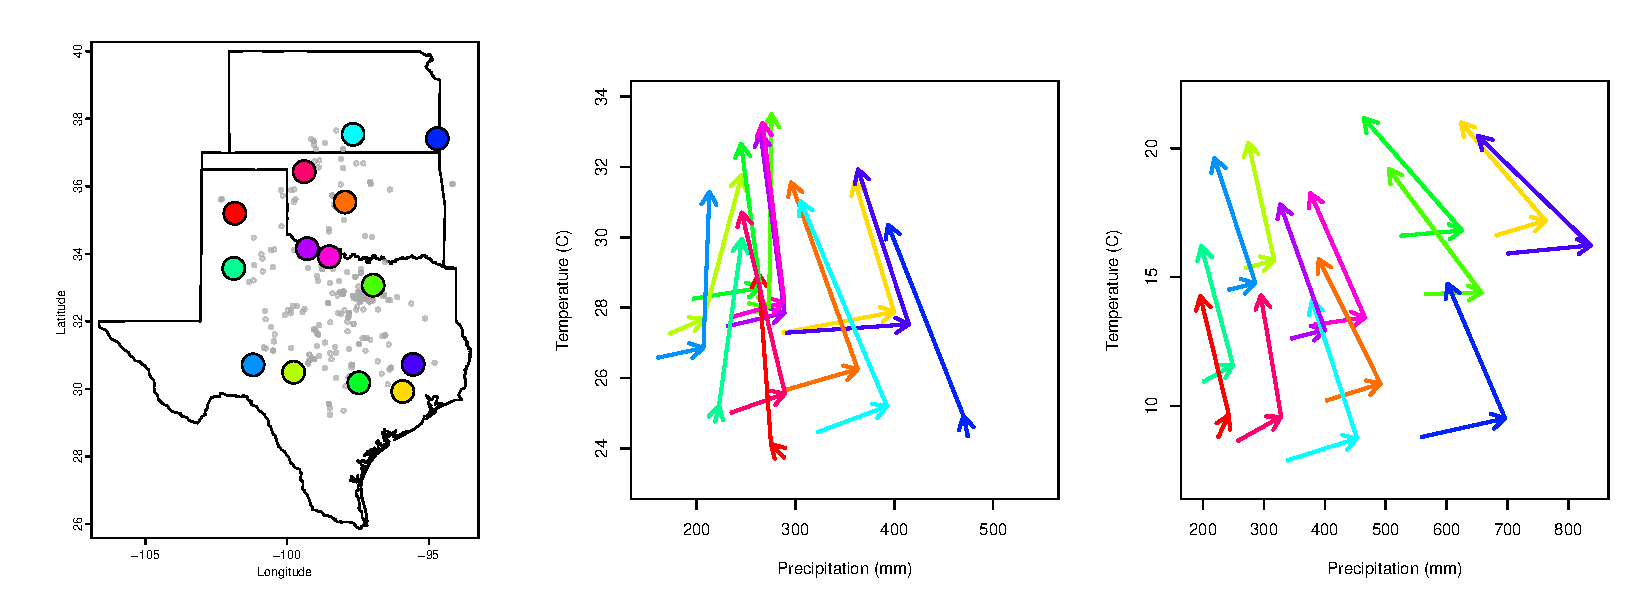
\includegraphics[width=1\linewidth]{tom_map_v1.pdf}
\caption{(A), Common garden locations in Texas, Oklahoma, and Kansas (points) and (B, C) corresponding changes in growing and dormant season climate. Arrows in B,C connect past (1901-1930) and present (1990-2019) climate normals, and present and future (2071-2100) climate normals under RCP4.5 and RCP8.5 forecasts. Future forecasts are from MIROC5 but other climate models show similar patterns.
			}
\label{fig:study_design}
\end{figure}
\clearpage

\begin{figure}[H]
\centering
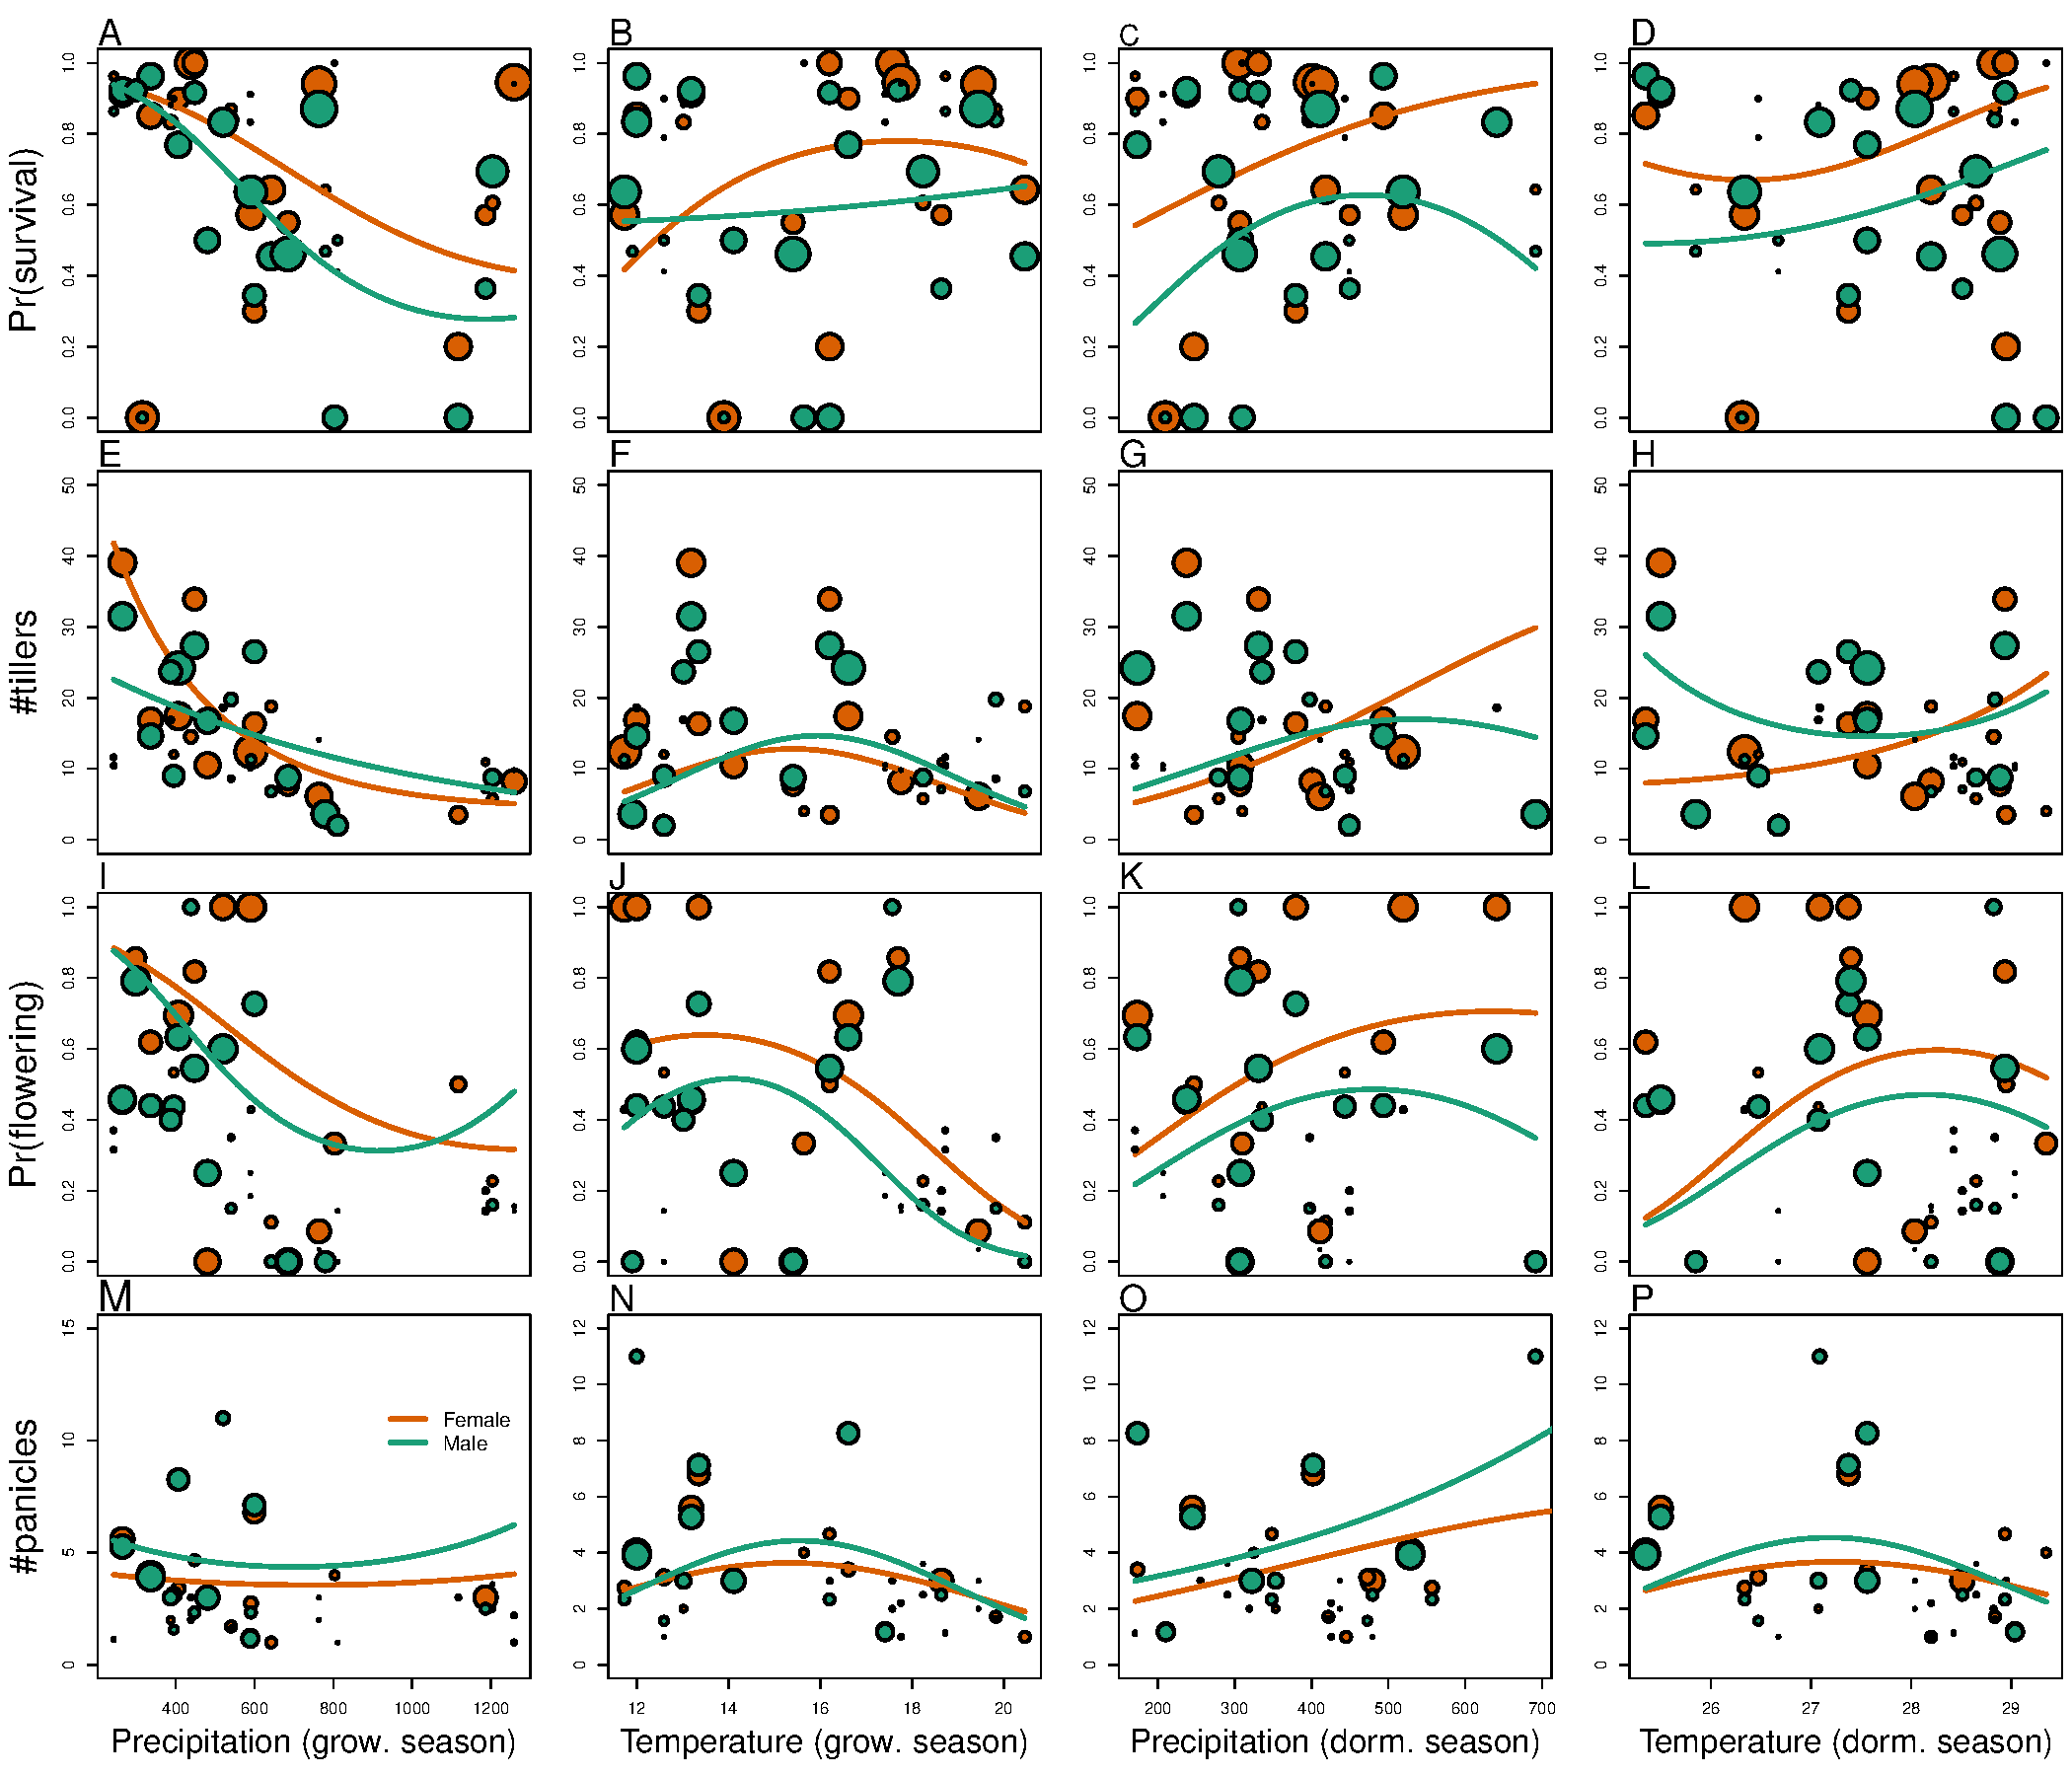
\includegraphics[width=1\linewidth]{vital_rates_v1.pdf}
\caption{Sex specific demographic response to climate across species range.
			% Vital rates as a function of each climatic variable given 3 others climate variables are constant.
			(A, B, C, D) Probability of survival as a function of precipitation and temperature of the growing and dormant season.
			% (C, D) Probability of survival during the dormant season conditional of climate average during the growing season.
			(E, F, G, H) Change in number of tillers as a function of precipitation and temperature of the growing and dormant season.
			% (F, G) Change in number of tillers during the dormant season conditional of climate average during the growing season.
			(I, J, K, L) Probability of flowering as a function of precipitation and temperature of growing and dormant season.
			% (K, L) Probability of flowering during the dormant season conditional of climate average during the growing season.
			(M, N, O, P) Change in number of panicles as a function of precipitation and temperature of the growing and dormant season.
			% (O, P) Change in number of panicles produced given flowering during the dormant season conditional of climate average during the growing season.
			Points show means by site for females (orange) and males (green). 
			Points sizes are proportional to the sample sizes of the mean and are jittered.
			Lines show fitted statistical models for females (orange) and males (green) based on posterior mean parameter values.
			%Lower panels below each data panel show the posterior distribution of the difference between females and males as a function of climate (positive and negative values indicate female and male advantage, respectively); dashed horizontal line shows zero difference.
			% Statistical results are shown in Figure \ref{Sup:Posterior}.
			The fitted lines were estimated using only one climate covariate, while the other covariates and size were held constant.
			}
\label{fig:vital_rates}
\end{figure}
\clearpage

\begin{figure}[H]
\centering
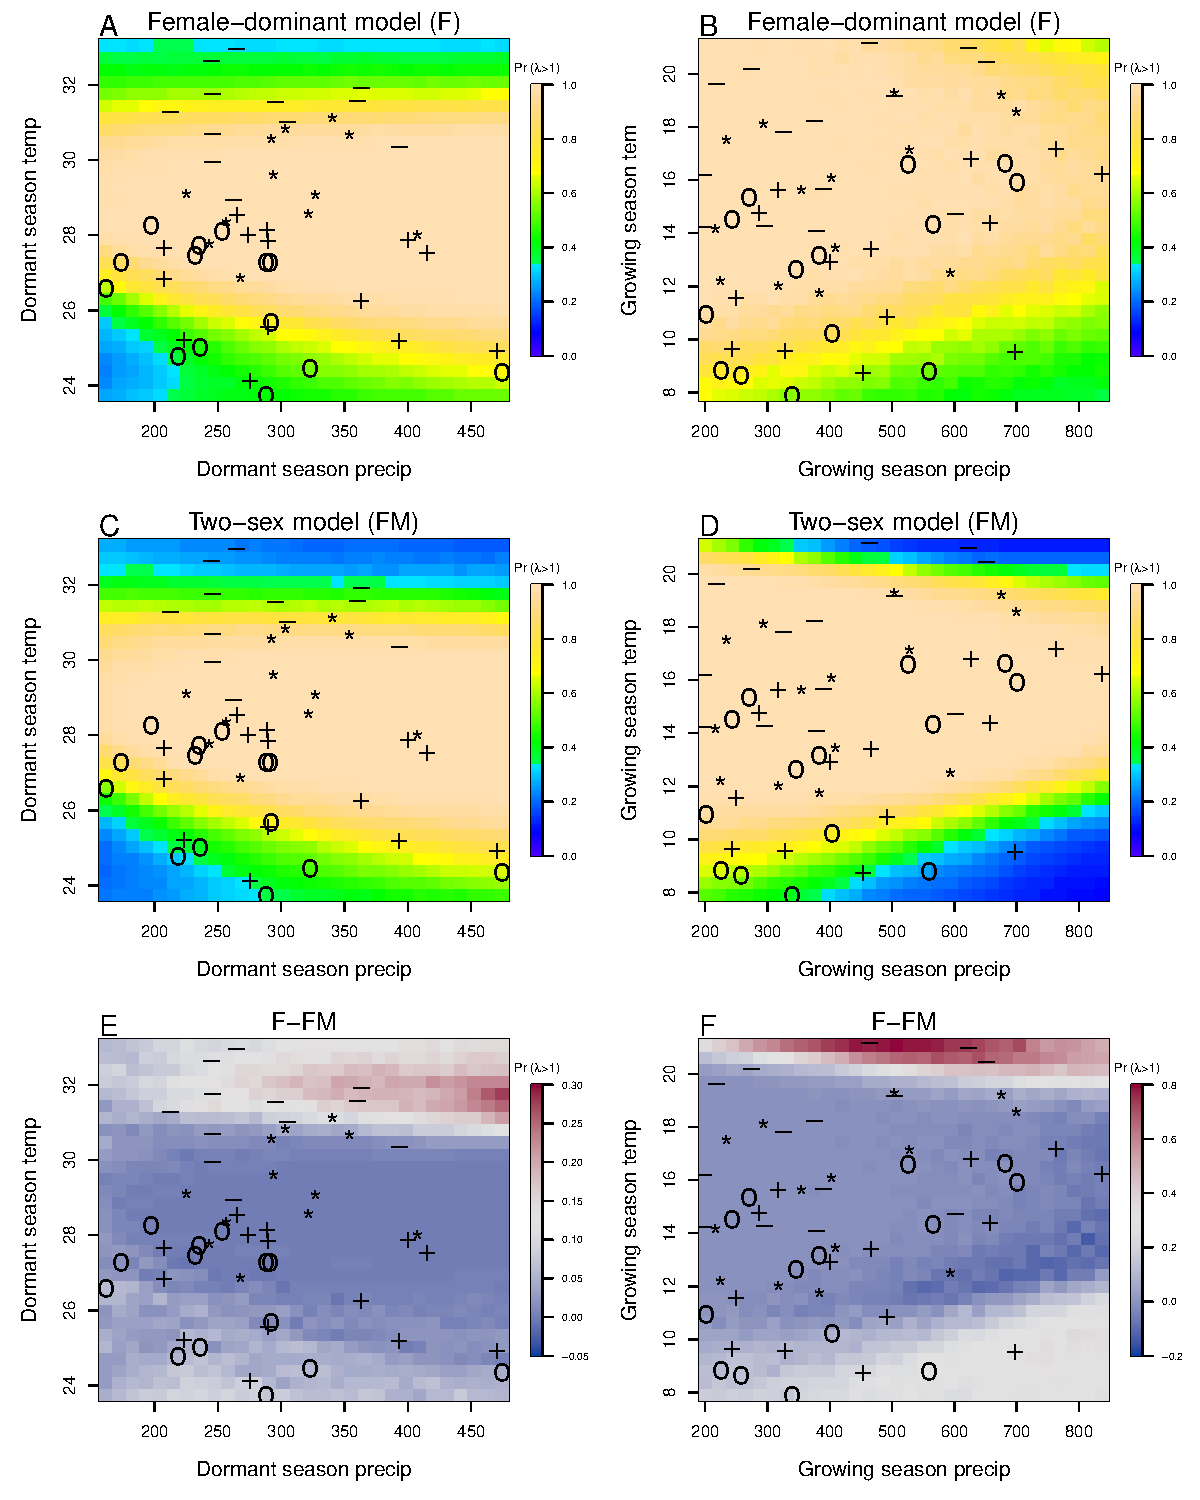
\includegraphics[width=1\linewidth]{niche_dormant_growing.pdf}
\caption{ A two‐dimensional representation of the predicted niche shift over time (past, present and future climate conditions). 
			(A, B, C, D)  show predicted probabilities of self- sustaining populations, Pr ($\lambda > 1$) conditional on precipitation and temperature of the dormant and growing season.
			% (A) Niche ( Pr ($\lambda$ > 1)) of dormant season for female dominant model, (B) Niche of growing season for female dominant model.
			% (C) Niche ( Pr ($\lambda$ > 1))of dormant season for the two sex model, (B) Niche of growing season for the two-sex model.
			(E, F) show difference in niche estimation between the female dominant model and the two-sex model for each season.
			"\begin{normalsize}\textbf{o}\end{normalsize}": Past, "\begin{normalsize}\textbf{+}\end{normalsize}": Current,"\begin{large}\textbf{*}\end{large}": RCP 4.5,"\begin{large}\textbf{-}\end{large}": RCP 8.5.
			}
\label{fig:niche}
\end{figure}
\clearpage

\begin{figure}[H]
\centering
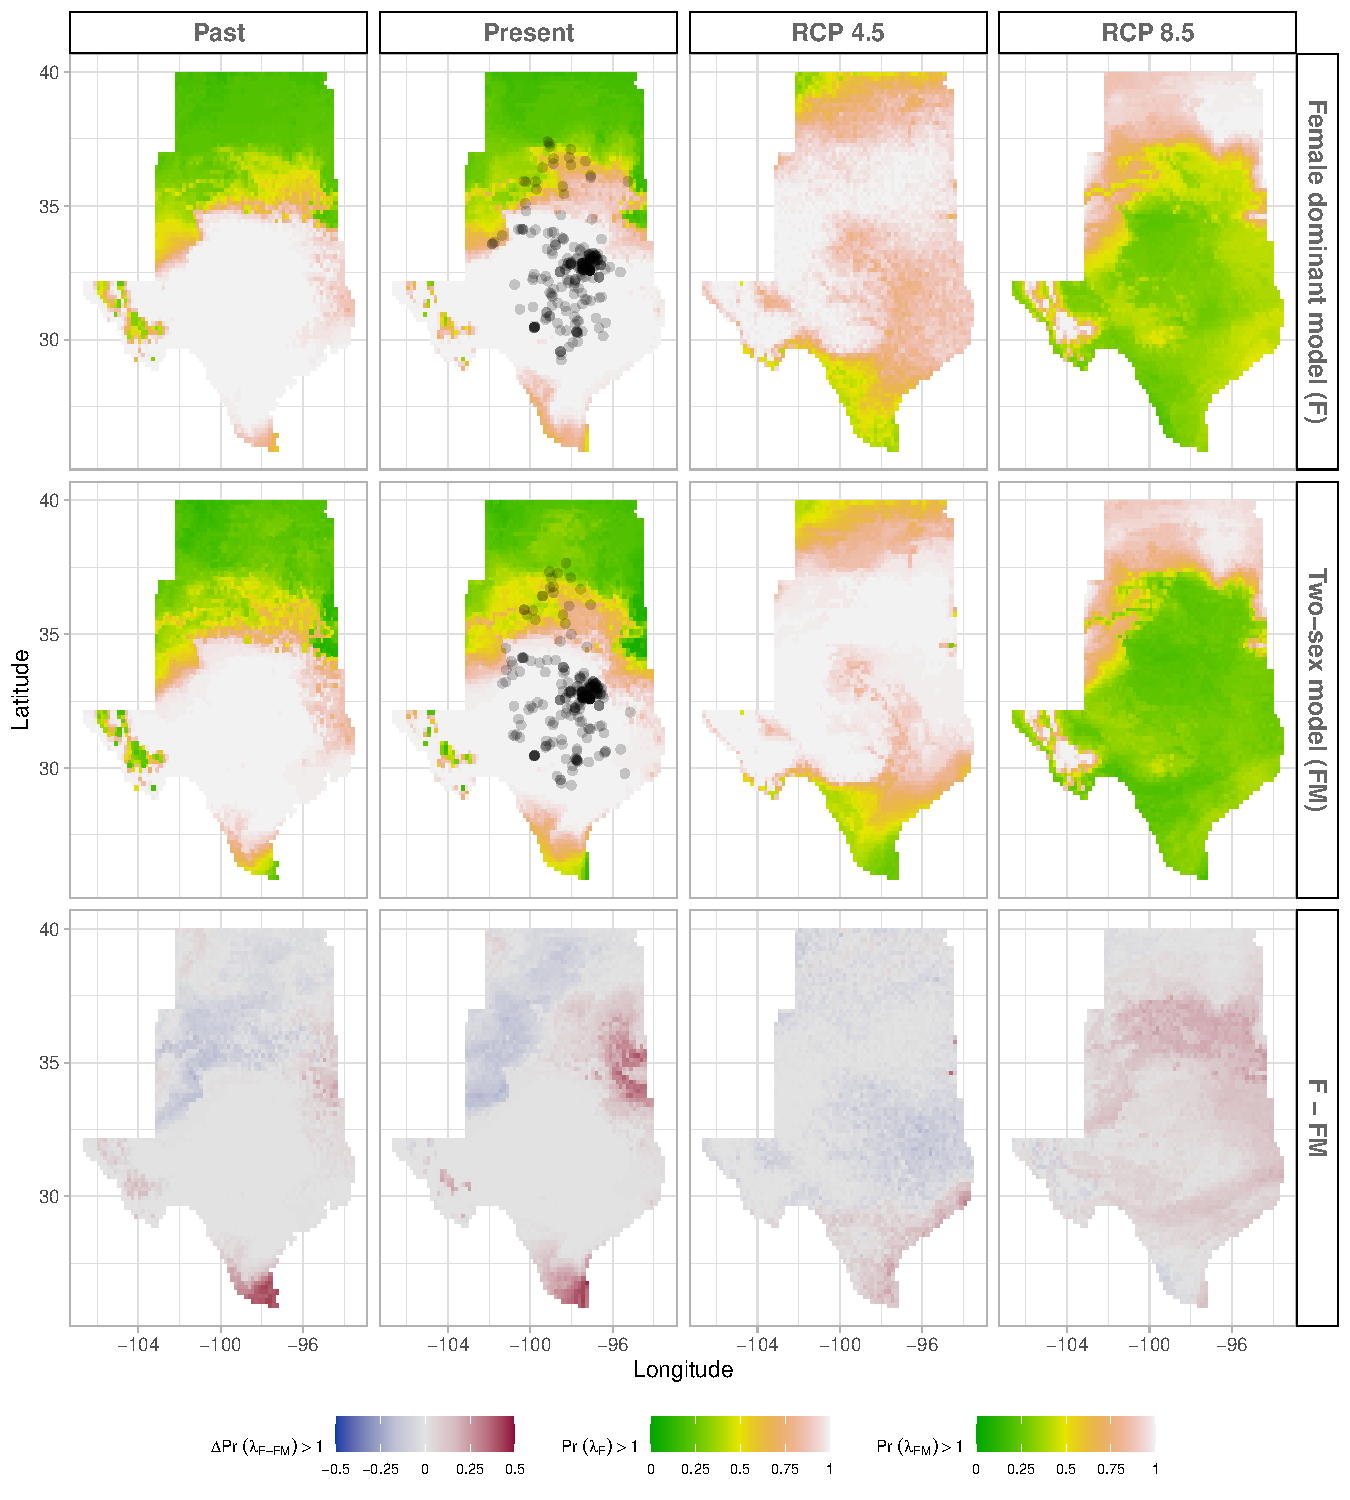
\includegraphics[width=1\linewidth]{Fig_geoPrlambdacmc.pdf}
\caption{ Climate change favors range shift towards north edge.
			(A) Past, (B) Current, (C and D) Future predicted range shift based on the predicted probabilities of self- sustaining populations, Pr ($\lambda > 1$), using the two-sex model that incorporates sex- specific demographic responses to climate with sex ratio dependent seed fertilization.
			(E) Past, (F) Current, (G and F) Future  predicted range shift based on the predicted probabilities of self- sustaining populations, Pr ($\lambda > 1$), using the female dominant model.
			Future projections were based on the CMCC-CM model.
			The black dots on panel B and F indicate all known presence points collected from GBIF. 
			The occurrences of GBIFs are distributed in with higher population fitness habitat Pr ($\lambda > 1$) , confirming that our study approach can reasonably predict range shifts. 
			}
\label{fig:geoprojcmc}
\end{figure}




\end{document}